\documentclass{article}%
\usepackage[T1]{fontenc}%
\usepackage[utf8]{inputenc}%
\usepackage{lmodern}%
\usepackage{textcomp}%
\usepackage{lastpage}%
\usepackage{authblk}%
\usepackage{graphicx}%
%
\title{Mitochondrial Dysfunction Promotes Breast Cancer Cell Migration and Invasion through HIF1a Accumulation via Increased Production of Reactive Oxygen Species}%
\author{Susan Avila}%
\affil{School of Medicine, Chung Shan Medical University, 110 Chien{-}Kuo N. Road, Section 1, Taichung 402, Taiwan}%
\date{01{-}01{-}2009}%
%
\begin{document}%
\normalsize%
\maketitle%
\section{Abstract}%
\label{sec:Abstract}%
Biology helps mammals seek food while bugs eat. What you may not know is that it is possible to aid in the process of colonization.\newline%
Researchers at Case Western Reserve University found that the Yersinia pestis Ail protein plays a critical role in the dispersal of infectious bacteria in and out of host cells. They report that the Yersinia pestis Ail protein acts as a route through which pathogenic bacteria enters host cells.\newline%
It is well known that the immune system interacts with bacteria within the body. The bacterial immune system replicates its defenses inside host cells and destroys the cells of the host cells of the pathogenic bacteria after they reach an immune cell hosting site (PC or viral host site).\newline%
A therapeutic approach is proposed to restore existing bacterial immune response if the pathogenic bacteria reach the host cell host site. In spite of the increased infection rate, other illnesses are significantly reduced (as little as a half percent in the absence of additional microbes).\newline%
The parasitic Yersinia pestis mollusks have an additional important role to play in the host bacterium that causes Sudden Infant Death Syndrome. Although SIDS was caused by common strains, the cases accounted for only 1.4 percent of all human deaths from suspected SIDS in 1980 (Read more). As the prevalence of Type II diabetes, increasing obesity, and obesity{-}related cancers have increased, the correlation between SIDS and Type II diabetes has evolved to include the causes.\newline%
For a newer SIDS investigation, an investigator engaged his team to determine if the Yersinia pestis Ail protein could be found at a site where SIDS affects SIDS and could be used as a new strategy for eradicating SIDS. The investigators collected patient samples from 122 U.S. infants that had died of SIDS from their birth to February 2001 (Read more).\newline%
In other applications, the protein, called Yatsenstadt{-}Norkenmendica, blocks infiltration of the pathogenic bacteria or viruses in the host cell from an infected pathogenic bacteria or virus without blocking all infiltration. The researchers tested the Yatsenstadt Norkenmendica which has been used to treat AIDS, hepatitis and SARS (2003). They found that the protein can efficiently bind to DNA and convert the X{-}rays present in a target cell into instructions for a specialized muscle system (Buymore 2010). They used the Yatsenstadt Norkenmendica to see if it could be used as a non{-}invasive control technique for treating SIDS.\newline%
The researchers examined Yatsenstadt{-}Norkenmendica in human host cells. They found that Yatsenstadt{-}Norkenmendica plays a key role in maintaining normal cell conformationsthe necessary mechanical condition to control the spread of abnormal viral DNA. They suggest that Yatsenstadt{-}Norkenmendica could be used in combination with other tools as a way to kill the infection by disinfecting the cell of the pathogenic bacteria or virus and providing sufficient therapeutic doses to eliminate the infected patient.

%
\subsection{Image Analysis}%
\label{subsec:ImageAnalysis}%


\begin{figure}[h!]%
\centering%
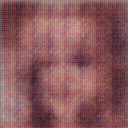
\includegraphics[width=150px]{500_fake_images/samples_5_348.png}%
\caption{A Black And White Cat Standing In A Forest}%
\end{figure}

%
\end{document}